\documentclass[11pt]{article}
\usepackage[utf8]{inputenc}
\usepackage{booktabs}
\usepackage{multicol}
\usepackage{amsmath}
\usepackage{amsfonts}
\usepackage{fullpage}
\usepackage{amsmath,amssymb,amsthm}
\usepackage{tikz,lipsum,lmodern}
\usepackage[most]{tcolorbox}
\usepackage{graphicx}
\def\R{{\mathbb{R}}}
\def\N{{\mathbb{N}}}


\begin{center}
    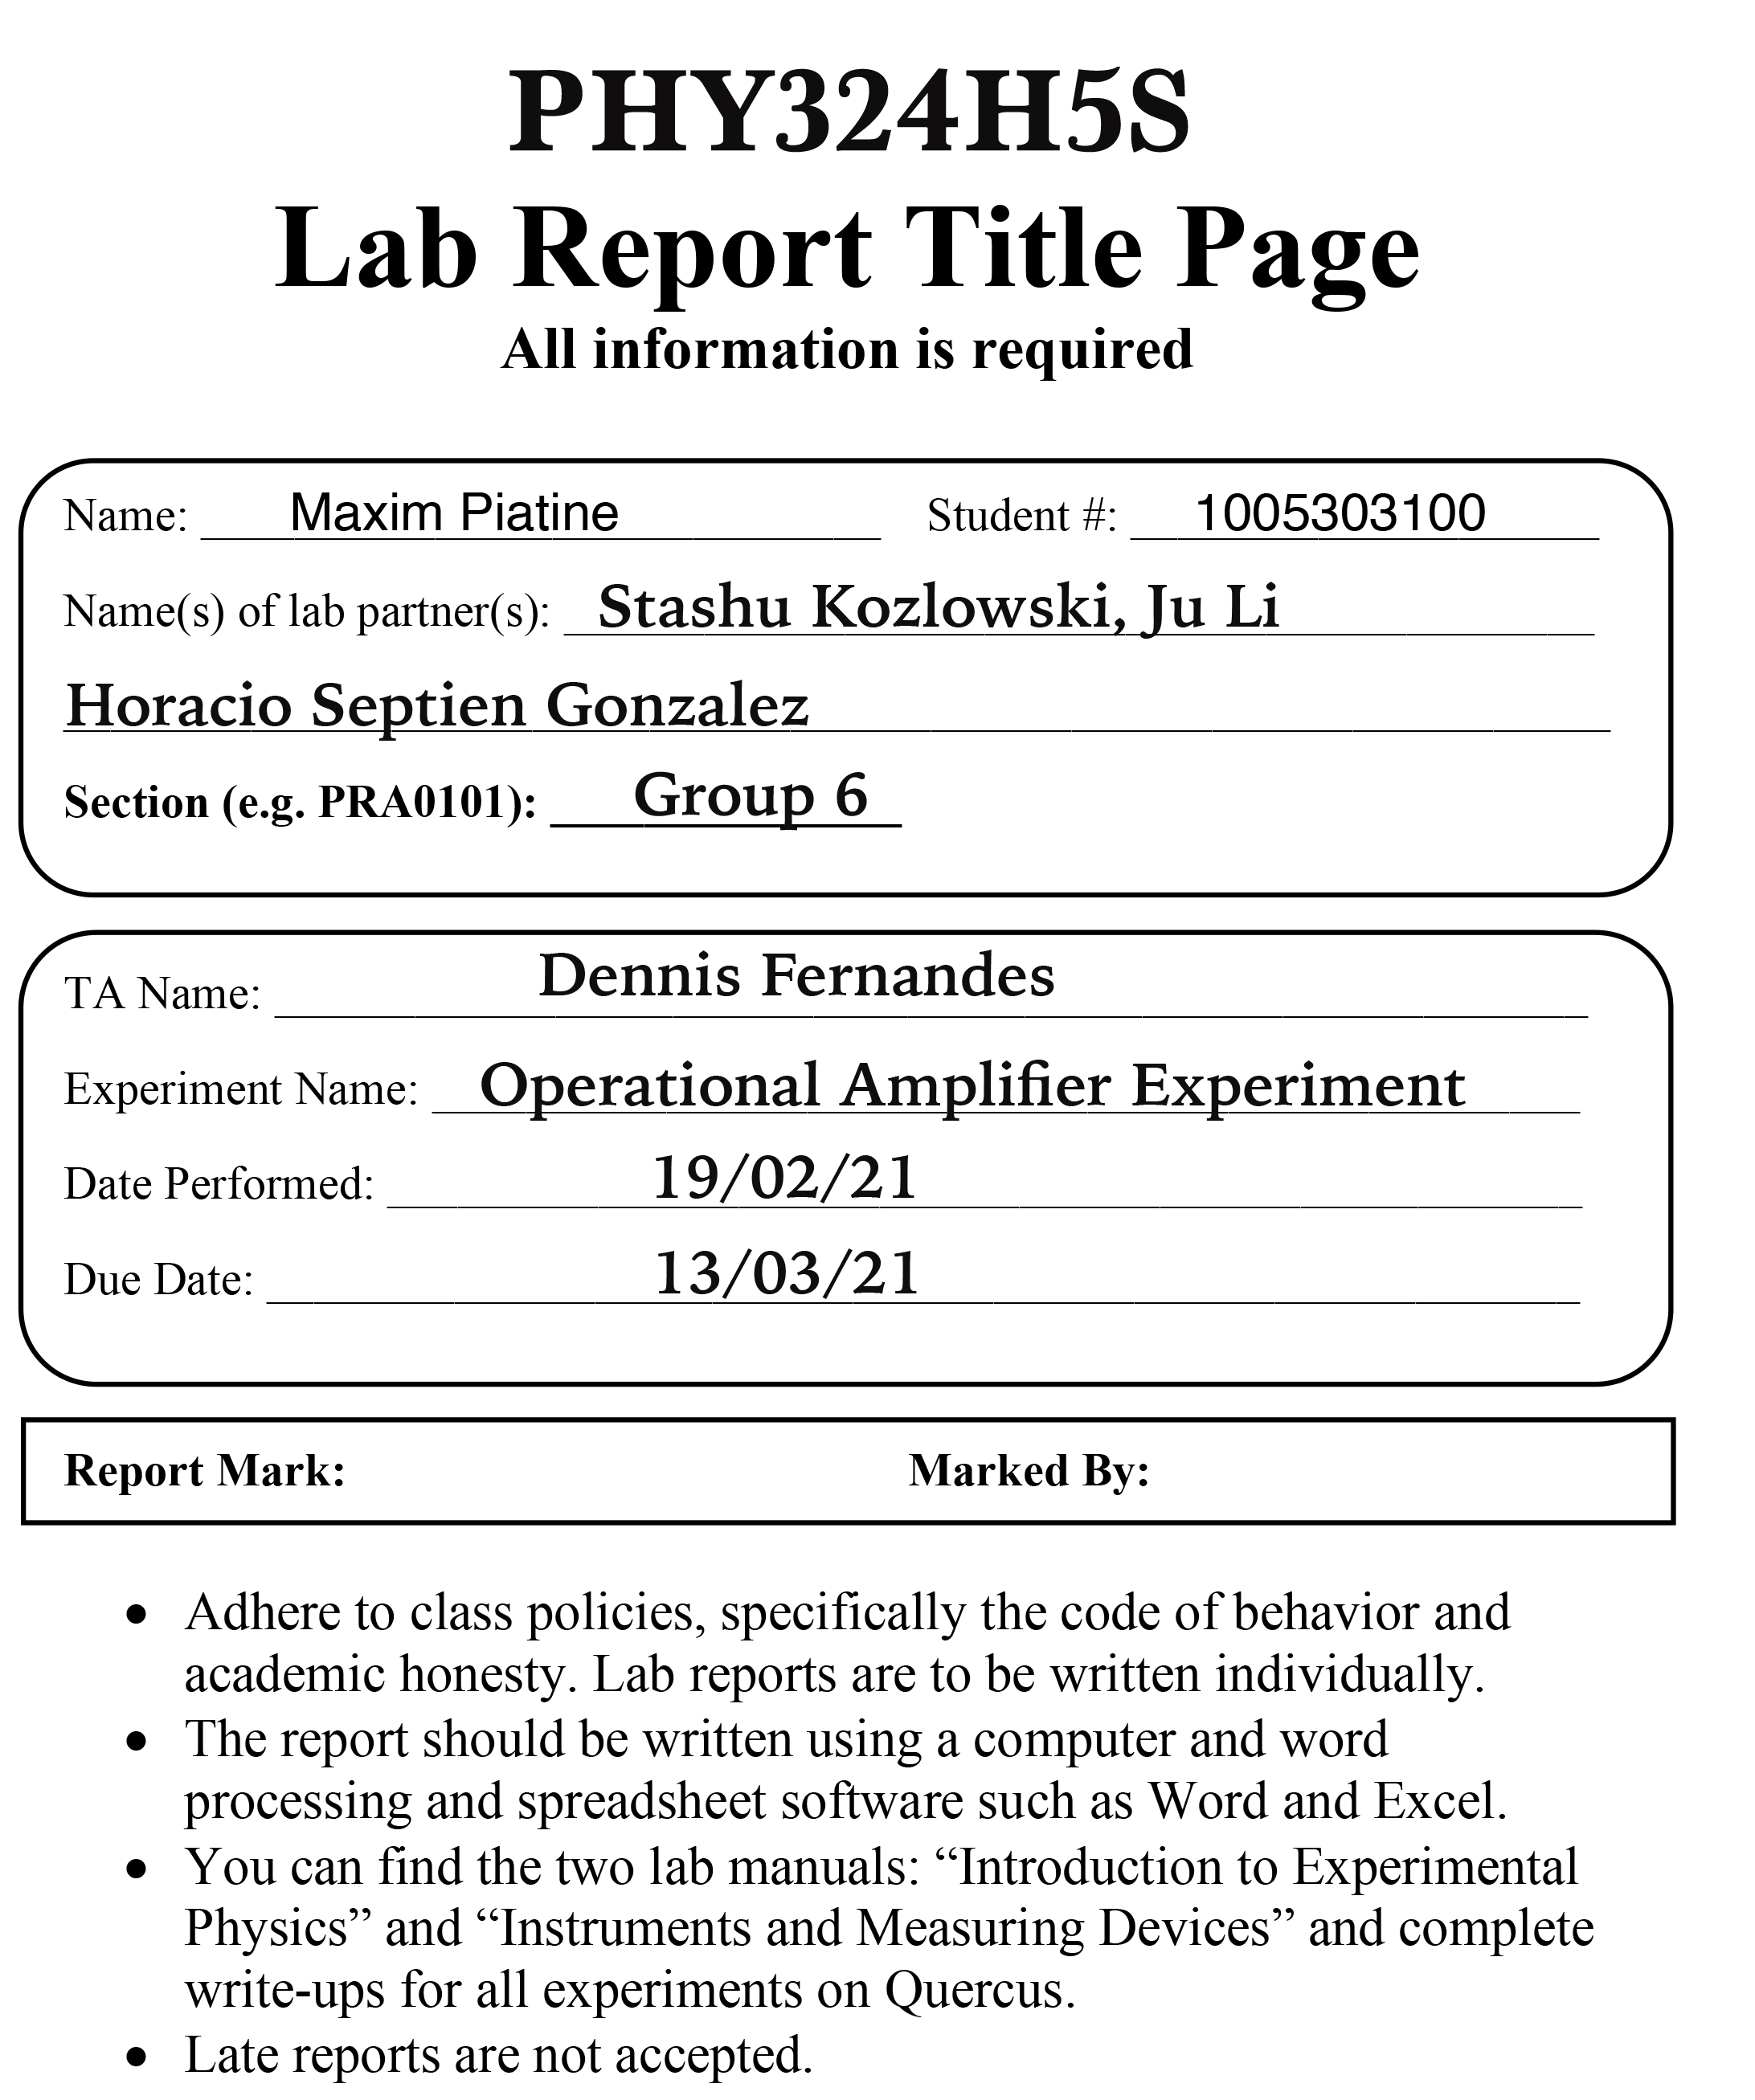
\includegraphics[width=17cm]{intro/OPAMP.png}
\end{center}

\newpage
\begin{document}
\section*{Abstract}
The  purpose  of  this  laboratory  activity  is  to  investigate  various  applications  of  op  amps,  specifically amplification, integration/differentiation, and addition/subtraction. Students will set up feedback networks with op amps and investigate the effects on the input signals at different frequencies. First, the experimental of the inverting and non inverting amplifier had a multiple step process with varying amounts of resistors and comparing them to the output voltage and input voltage. From the collection of computation found in appendix table 1, the average error percentage of the inverting experiment was $0.8\%$, and for the non-inverting circuit the error percentage was $1\%$ from the comparison of voltages and resistances. Reason for the voltage and resistances comparison was to determine the gain of amplitudes the inverting and non-inverting circuits were having from the theoretical equations (7) and (10).\\
Finally, investigating the inverted differentiator and integrator, provided insight on the output voltages determined by equations (16) and (22). The inverted differentiator, the experimental output voltage followed the same graph as the computational sinusoidal function determined via matlab. Deriving the equation of the output voltage as the derivative of the sine function. The inverted integrator, using the integral of the input function provided insight on the output voltage. Using the theoretical knowledge of an integral, the area under the curve between both input and output voltage gave a $39\%$ error. The integral of the input voltage was $-0.012V$ and the output voltage was $-0.019V$. The experimental outcomes of this laboratory followed well with the theory of op amps. 

\section*{Introduction}
Op Amps, also known as Operational Amplifier, is a cheap integrated circuit that can be used as a building block of electronics. It is an amplifier with a large open loop gain. It has an inverting input and a non-inverting input, and a single output. The relationship between the input and the output depends upon the feedback network that connects them.\\
An op amp performs operations on an input signal. Some of the possible operations include amplification, buffering, integration, differentiation, addition, and subtraction. When used in an open loop, the op amp has poor stability and very high gain (infinite for an ideal op amp). In a closed loop, the feedback adds stability and reduces the gain of the amplifier.
\begin{center}
    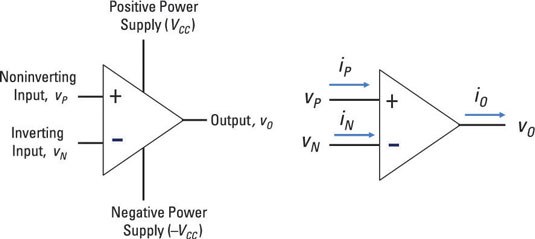
\includegraphics[width=10cm]{intro/2.jpg}\\\textbf{Figure 1}: In an op amp there is always a positive voltage input and a negative voltage input. An op amp with – (inverting) and + (non-inverting) inputs. If the positive voltage input is up, then the voltage output is positive. If the negative voltage input is up, then the voltage output is negative. Inverting symbols go in the opposite directions and Non-inverting doe the opposite. Current for an ideal op amp is zero.  
\end{center}
First rule:
\begin{equation}
    V_1=V_2
\end{equation}
the op amp changes its output to lower the voltage difference between its inputs to zero.\\
Second rule
\begin{equation}
    I_1=I_2=0
\end{equation} 
the inputs draw no current and are essentially connected to an open circuit. 
\\The resulting output from voltage applied within both voltages:
\begin{equation}
    V_o=A(V^+ - V^-)
\end{equation}
\begin{equation}
    V_o=AV_{in}
\end{equation}
In an op amp, based of equation(2), makes the output voltage:
\begin{equation}
    A=\frac{V_o}{V_{in}}
\end{equation}
Based of that, the amplifier will be able to change the voltage of the output compared to the input. Since the amplifier is connected to the power supply; thus, accounting for the difference of energy of input and output. The amplifier is connected to the positive and negative power supply.\\

\\Inverting amplifier comes from the input of inverting, where the negative charge goes through this Figure 2. 
\begin{center}
    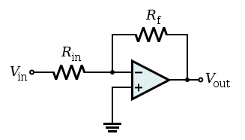
\includegraphics[width=7cm]{intro/3.png}\\\textbf{Figure 2}: This is an inverting amplifier circuit.
\end{center}
The output of the inverting amplifier is equal to $-\frac{R_f}{R_{in}}$ times the input signal since the negative input is high. The input of op amps draws no current; meaning that the current flowing in resistor $R_{in}$ and $R_f$ is the same. With the help of Ohm's law:
\begin{equation}
    \frac{V_o}{R_f}=\frac{-V_{in}}{R_{in}}
\end{equation}
\begin{equation}
    A=\frac{V_o}{V_{in}}=\frac{-R_f}{R_{in}}
\end{equation}

The non-inverting amplifier is opposite to the inverting one. The input resistor $R_1$ is grounded. Following rules (1) and (2), (2) tries to drive the current to zero at the intersection between $R_1$ and $R_2$ (Figure 3), and (1) makes the voltage equal to the input voltage. Leading to:
\begin{equation}
    \frac{V_{in}}{R_1}=\frac{V_{o}-V_{in}}{R_2}
\end{equation}
\begin{equation}
    \frac{R_2}{R_1}=\frac{V_{o}-V_{in}}{V_{in}}=\frac{V_{o}}{V_{in}}-1
\end{equation}
\begin{equation}
    A=\frac{V_{o}}{V_{in}}=\frac{R_2}{R_1}+1
\end{equation}
\begin{center}
    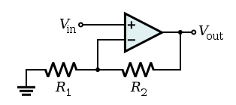
\includegraphics[width=7cm]{intro/4.png}\\\textbf{Figure 3}: A non-inverting amplifier circuit. The input resistor $R_1$ is grounded.
\end{center}
Inverting Differentiator or differentiating amplifier consists of capacitor $C$ at the input and a resistor $R$. The current flowing through the capacitor $C$ is given by:
\begin{equation}
    I=C\frac{dV}{dt}=C\dot V
\end{equation}
Where $I$ is the current through capacitor, $V$ is the voltage across the capacitor, and $dV/dt$ is the rate of change through the capacitor.\\
The current can also be represented with ohm's law:
\begin{equation}
    I=\frac{V}{R}
\end{equation}
Using the current law equation (2)
\begin{equation}
    I_o=I_{in}
\end{equation}
\begin{equation}
    I_o=\frac{0-V_o}{R} \text{ and } I_{in}=C\frac{dV_{in}}{dt}
\end{equation}
\begin{equation}
    \frac{-V_o}{R}=C\frac{dV_{in}}{dt}
\end{equation}
\begin{equation}
    V_o=-RC\frac{dV_{in}}{dt}
\end{equation}
There will be some small resistance $R_{in}$ in series with the capacitor, and the differentiator will only work at frequencies below $\omega_C=\frac{1}{R_{in}C}$.
\begin{center}
    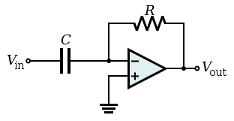
\includegraphics[width=7cm]{intro/figure4.png}\\\textbf{Figure 4}: An idea inverting differentiator circuit.
\end{center}
Inverting Integrator consists of resistor $R$ at the input and a capacitor, the reverse of the differentiating amplifier. Same principle as the inverting differentiator, the intersection/node between the resistor and amplifier, the potential at the node is zero. Using current law:
\begin{equation}
    I_{in}=I_o
\end{equation}
\begin{equation}
    I_{in}=\frac{V_{in}-0}{R}=\frac{V_{in}}{R}
\end{equation}
The current over the capacitor is similar to the differentiating amplifier:
\begin{equation}
    I_o=C\frac{d(0-V_o)}{dt}=-C\frac{dV_o}{dt}
\end{equation}
\begin{equation}
    \frac{V_{in}}{R}=-C\frac{dV_o}{dt}
\end{equation}
\begin{equation}
    -\frac{V_{in}dt}{RC}=dV_o=\int^{V_o}_0dV_o=V_o
\end{equation}
\begin{equation}
    V_o=-\frac{1}{RC}\int^t_0 V_{in} dt
\end{equation}
\begin{center}
    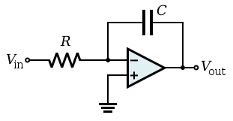
\includegraphics[width=7cm]{intro/figure5.png}\\\textbf{Figure 5}: An ideal inverting integrator circuit.
\end{center}
The behavior of the device can be improved by adding a resistor $R_f$ in parallel with the capacitor. This does not come without a tradeoff, however, as it prevents the circuit from integrating at all frequencies. In practice, with the resistor in place, the integrator will work at frequencies above $\omega_C=\frac{1}{R_fC}$.

\section*{Procedure}
The experiment will need to use resistors. Thus, measuring the resistors appropriate for the experiment. Manual suggests resistors of $10k\Omega$ and $100k\Omega$ for the inverting and non-inverting amplifiers. Furthermore, measure the capacitance as well for the inverting differentiator and inverting integrator. Making sure that the value is $10nF$.\\
After measuring the important informations, the manual shows a breadboard.
\begin{center}
    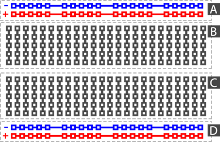
\includegraphics[width=7cm]{bread.png}\\\textbf{Figure 6}: The wiring layout of a standard electronics breadboard.
\end{center}
The first two rows are connected horizontally and are often used as $+5V$ rail and a ground rail. The next five rows are connected vertically and not horizontally. Both groups of 5 rows from B and C are separated by a channel that is a proper width to install an integrated circuit. The last 2 rows are connected horizontally same as A.\\
Using the breadboard to set up the inverted amplifier circuit connect the resistors to the corresponding areas and connect the ground wire to one of the posts.\\
Lastly, connecting the wires from the breadboard posts to the oscilloscope to receive information regarding the sinusoidal waves obtained. The input and output voltage will resemble a sinusoidal wave. The oscilloscope can save all the data and graphs; however, adjust the graphs to fit properly with the analogues.\\

\\Changing from the inverting and non-inverting amplifiers to inverting differentiator and inverting integrator, most of the circuit remains intact except for some minor adjustments. The oscilloscope will provide the graphs on the input and the output of the voltage. The output voltage will be the derivative or the integral depending on how the circuit is set up; depending on the inverting differentiator or inverting integrator. Finally, save all the data for different wave shapes.

\section*{Data and Analysis}
The experiment allowed us to investigate various applications of operational amplifier and its applications. Amplification, integration/differentiation, and addition/subtraction. Building and simulating some op amps circuits. \\
One of the applications that is being tested is the inverting and non-inverting amplifiers. Like explained in the theory, the circuits are opposite in construction and they're wavelengths are the opposite as well. The frequency and amplitude used in this experiments are $145 Hz$ and $500 mV$ respectively. If the frequency is increased then the op amp will not be able to keep up making the amplitude output; therefore, the output voltage will decrease.\\
Firstly, the inverted amplifier data was collected through different selected tasks. The first three measurements are from the initial resistor of $10.6 k\Omega$ remaining constant and final resistor fluctuating, then the three last measurements kept the final resistor as constant at $47.1 k\Omega$ and the initial fluctuating (Table 1 in Appendix). 
\begin{center}
    \textbf{Graph 1}: Oscilloscope Graphical Image of Inverted Amplifier
    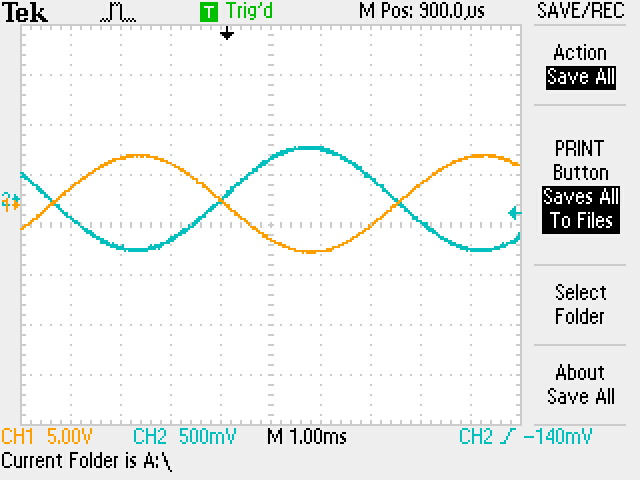
\includegraphics[width=7cm]{1st analysis/F0000TEK.JPG}\\\textbf{Graph 1}: An example of the oscilloscope graph. The independent axis $x$ is given by time in seconds. The dependent axis $y$ is given by the voltage. The orange oscillation graph, channel 1, is the output voltage. The teal oscillation graph, channel 2, is the input voltage. The output and input voltage oscillations have opposite oscillations. These graphs and inputs are used to compute the experimental gain for this laboratory. 
\end{center}
\newpage
\begin{center}
    \textbf{Graph 2}: Different Output Voltages from Resistances to Input Voltage in Inverted Amplifier\\
    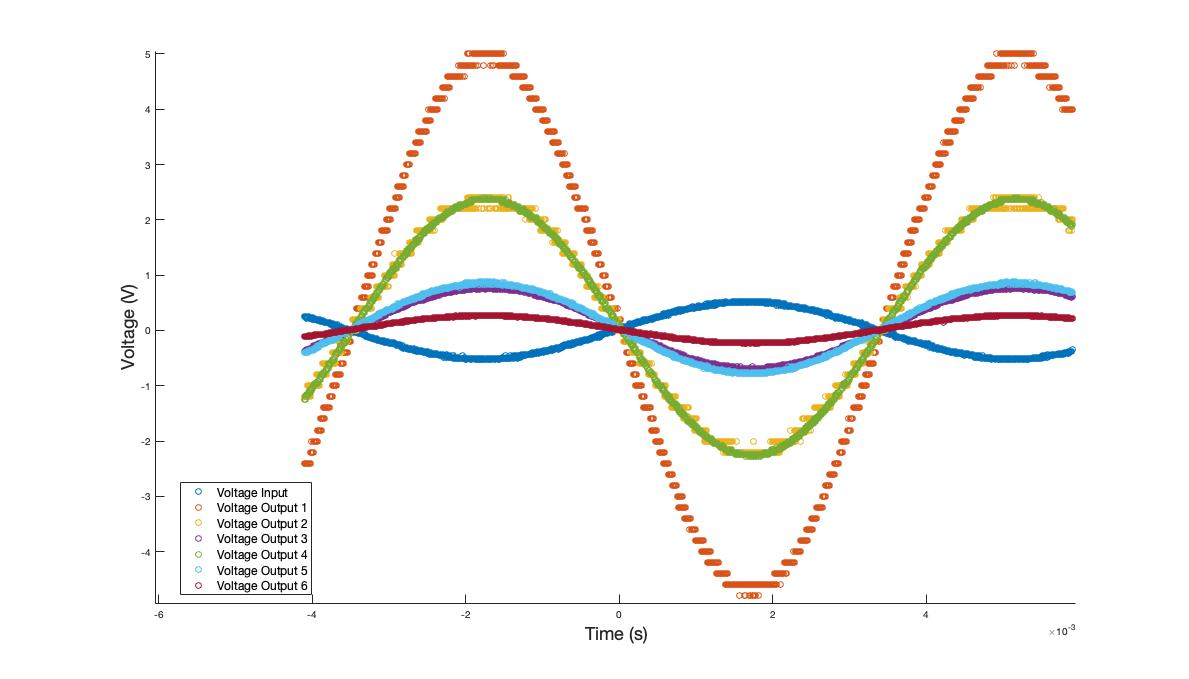
\includegraphics[width=15cm]{1st analysis/everything.jpg}\\\textbf{Graph 2}: Oscillations of different voltages with different resistors used. The independent axis $x$ is given by time in seconds. The dependent axis $y$ is given by the voltage. Six out of seven oscillations are due to the different resistances inverting the graph comparing to the input voltage. The input voltage is the only blue graph that follows a different oscillation than the rest of the graphs. The orange, yellow, lime, baby blue, and burgundy colours follow a sinusoidal type of oscillation, while the input voltage follows a negative sinusoidal oscillation. 
\end{center}
A suitable way of determining the gain of the amplitudes is by plotting a graph of output amplitude in respect to input amplitude. With the theoretical calculations that can be done with equation (7), the theoretical gain can be calculated. Using the first resistor of the inverting amplifiers, the initial resistor and the final resistor have values of $10.57 k\Omega$ and $98.1 k\Omega$, giving a theoretical gain of $-9.28$. The experimental value of gain obtained in Graph 3 is compared to the theoretical value. The experimental gain of the first resistance is $-9.39$, giving an error percentage of $1.21\%$.
\newpage
\begin{center}
    \textbf{Graph 3}: The Experimental Gain for All Resistors in Inverted Amplifier\\
    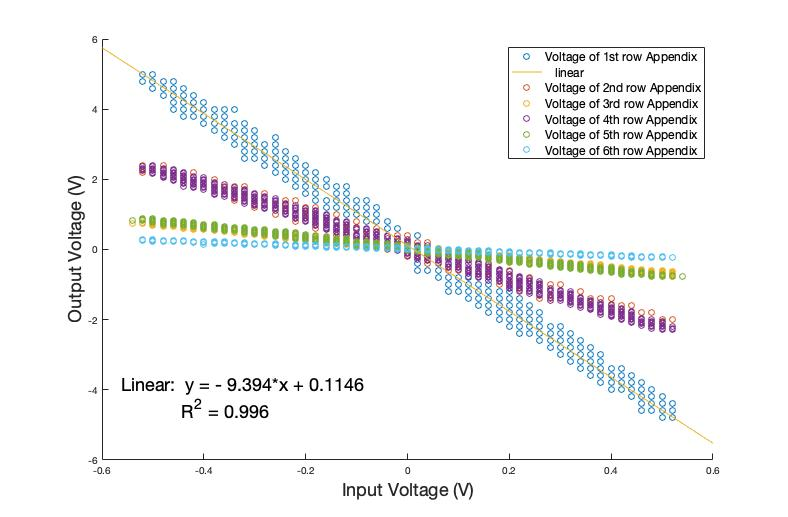
\includegraphics[width=12cm]{1st analysis/finalyes.jpg}\\\textbf{Graph 3}: From the raw data collected. The independent value is the input amplitude provided for each resistor. The dependent value is the output amplitude provided for each resistor. There were a total of six resistors attempts with three different final resistors and three different initial resistors. The slope of the first gain is $-9.394$, which is the experimental gain from the first resistors. The other experimental and theoretical gains are listed in the appendix (Table 1). The $R^2$ of this graph is $0.996$, indicating that the data is $99.6\%$ of the variation in the $y$ data is due to the variation in the $x$ data; indicating a perfect relationship between all the points. The rest of the linear correlations are above $99\%$ making all the data points in perfect variation of each other.
\end{center}
The non inverted amplifier tested the theoretical and experimental gain with theoretical equation (10). Since the inverted had a negatively measured result, the non-inverted is expected to be positive due to the initial voltage being positive. The same resistances processes from the inverted circuit is used for this part of the experiment.
\newpage
\begin{center}
    \textbf{Graph 4}: Different Output Voltages from Resistances to Input Voltage in Non Inverted Amplifier\\
    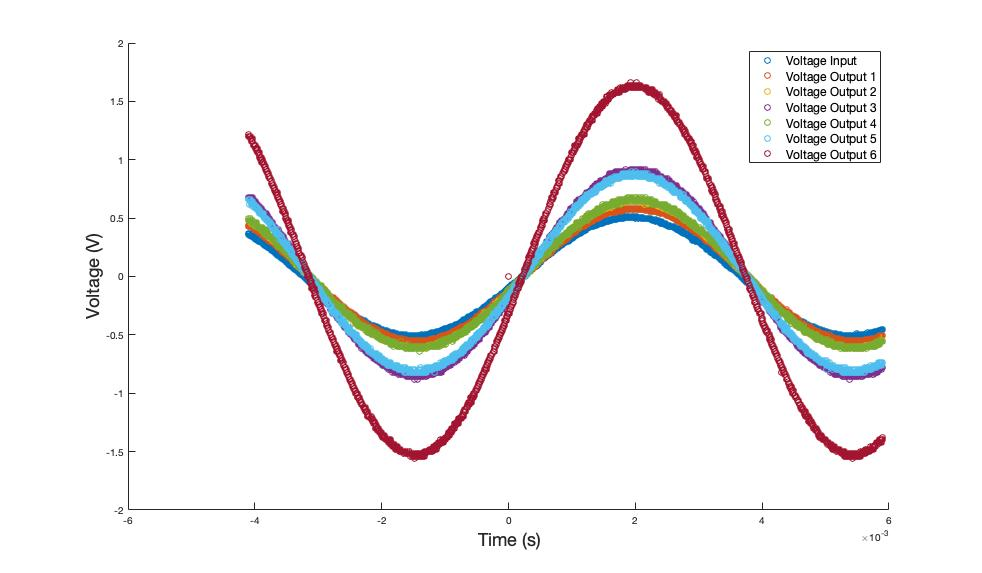
\includegraphics[width=14cm]{all.jpg}\\\textbf{Graph 4}: Oscillations of different voltages with different resistors used. The independent axis $x$ is given by time in seconds. The dependent axis $y$ is given by the voltage. Six out of seven oscillations are due to the different resistances. The input voltage is the blue graph that follows the same oscillations as the rest.
\end{center}
\begin{center}
    \textbf{Graph 5}: The Experimental Gain for All Resistors in Non Inverted Amplifier\\
    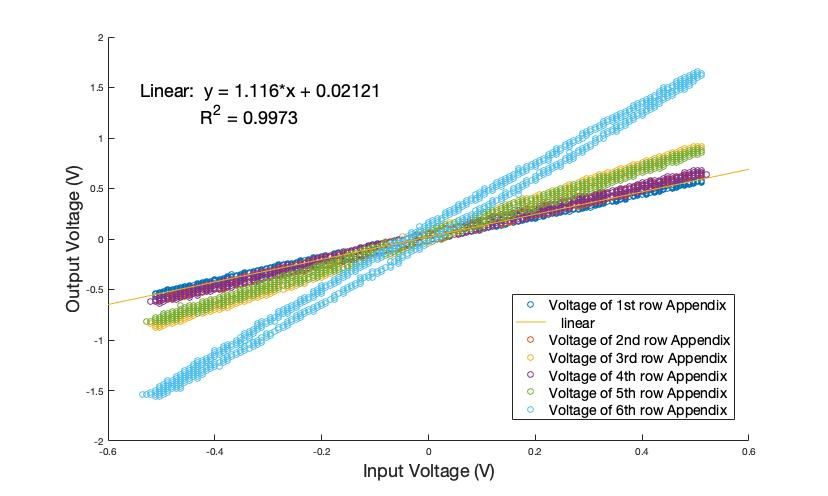
\includegraphics[width=11cm]{2nd.jpg}\\\textbf{Graph 5}: From the raw data collected. The independent value is the input amplitude provided for each resistor. The dependent value is the output amplitude provided for each resistor. There were a total of six resistors attempts with three different final resistors and three different initial resistors. The slope of the first gain is $1.12$, which is the experimental gain from the first resistors. The other experimental and theoretical gains are listed in the appendix (Table 2). The $R^2$ of this graph is $0.997$, indicating that the data is $99.7\%$ of the variation in the $y$ data is due to the variation in the $x$ data; indicating a perfect relationship between all the points. The rest of the linear correlations are above $99\%$ making all the data points in perfect variation of each other.
\end{center}
Based on all the computational results done in the appendix, the experimental and theoretical values are withing $1\%$ of error percentage. Meaning, the equation (10), the output voltage and the input voltage correspond to the ratio between resistors to be the gain of the amplifier. Taking the first resistors to compute the gain, $R_1=98.1 k\Omega$ and $R_2=10.57 k\Omega$, provided a ratio of $1.1$, comparing to the experimental voltage output over voltage input of $1.11$. Giving an error percentage of $0.71\%$.\\

\\Secondly, The inverting differentiator follows the theoretical procedure of equation(16). Where the output voltage is represented by the $-RC$ times the derivative of the initial voltage. By setting up the circuit with a feedback resistor in parallel with the capacitor, it allows the feedback resistor to set operating voltage point and controls the amount of output. 
\begin{center}
    \textbf{Graph 6}: Oscilloscope Graphical Image of Inverted Differentiator
    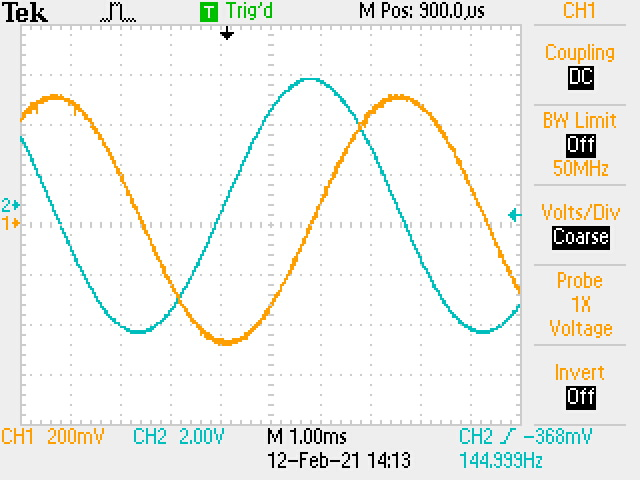
\includegraphics[width=7cm]{Differentiator/F0012TEK.JPG}
    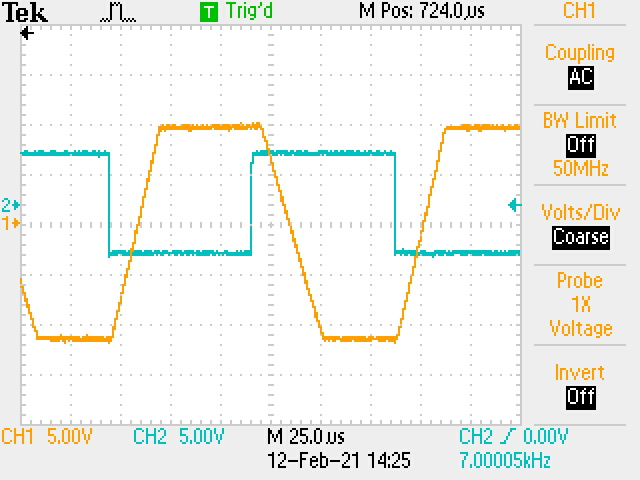
\includegraphics[width=7cm]{Differentiator/F0015TEK.JPG}
    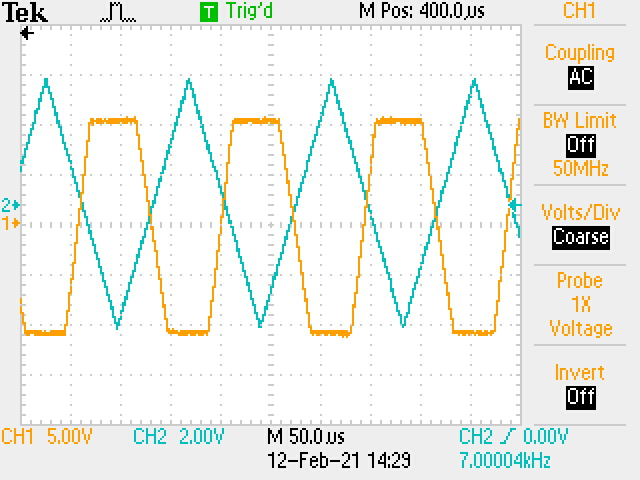
\includegraphics[width=7cm]{Differentiator/F0017TEK.JPG}\\\textbf{Graph 6}: The collected oscilloscope graphs are represented as sine wave top left, square wave top right, triangle wave on the bottom. Where the input of the graph becomes the derivative of the output. The blue graphs, channel 2, is the input. The orange graphs, channel 1, is the output. The independent value is the time and the dependent time is the voltage. 
\end{center}
\newpage
\begin{center}
    \textbf{Graph 7}: Experimental Output and Input Voltage of an Inverted Differentiator
    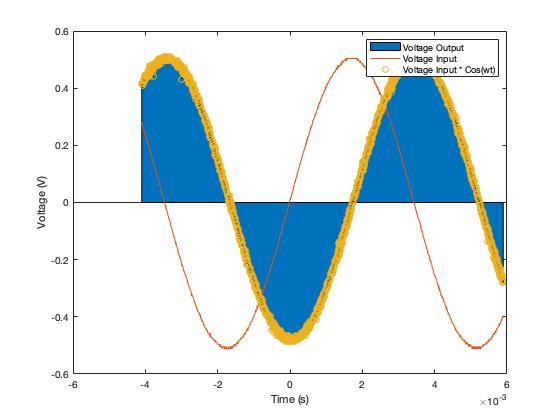
\includegraphics[width=10cm]{derivative.jpg}\\\textbf{Graph 7}: From the collected raw data, this graph was constructed with the independent value $x$ being the time measured in seconds and the dependent value $y$ being the voltage. The blue area graph is the voltage output, the orange graph is the voltage input, and the yellow graph is the calculated graph from the input voltage (Calculation in Appendix). 
\end{center}
To confirm the theory of inverting differentiator, equation (16), the output voltage is equal to the $-RC$ of the derivative of the input. Based on the calculation done and code created in matlab, the derivative of the input times the resistance and capacitance gave the voltage output predicted. Looking at Graph 7, the yellow graph being the computed derivative of the sinusoidal wave $V_{in}sin(\omega t)$, is the equivalence of the output voltage wave. Since the input wave is a sinusoidal graph, the output followed a cosine function.\\

\\The inverting integrator follows the theoretical procedure of equation(22). Where the output voltage is represented by the $\frac{1}{-RC}$ times the integral of the initial voltage. The inverting integrator follows a similar process as the inverted differentiator, but in a integral fashion.
\newpage
\begin{center}
    \textbf{Graph 8}: Oscilloscope Graphical Image of Inverted Integrator
    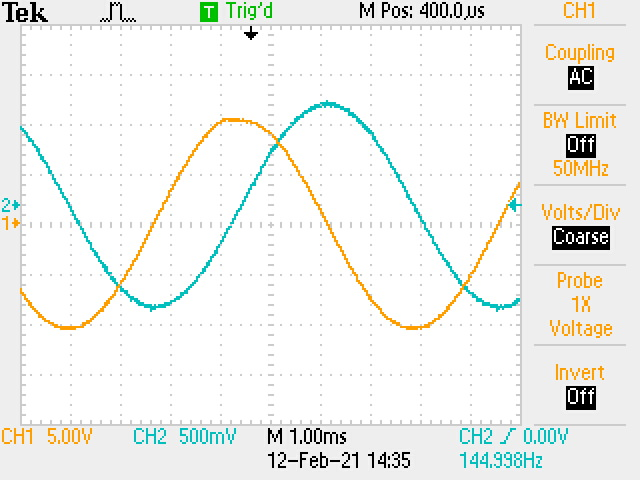
\includegraphics[width=7cm]{Integrator/F0018TEK.JPG}
    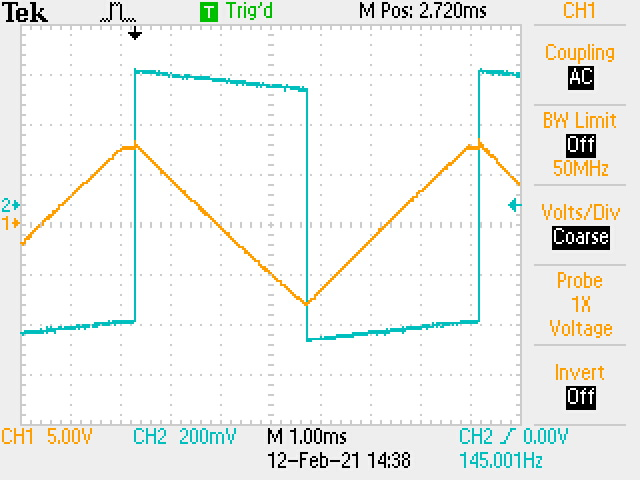
\includegraphics[width=7cm]{Integrator/F0020TEK.JPG}
    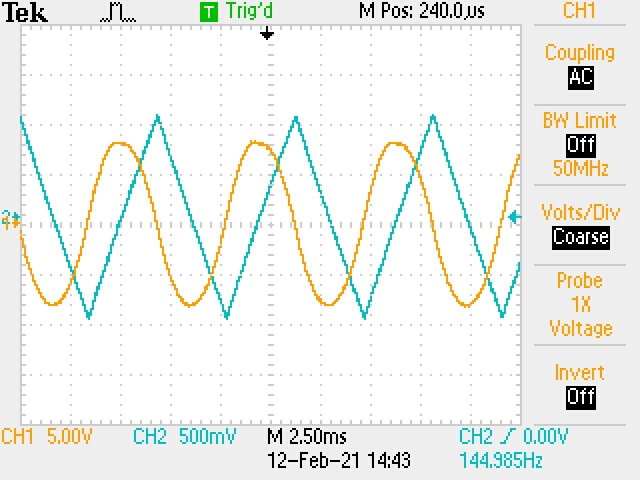
\includegraphics[width=7cm]{Integrator/F0022TEK.JPG}\\\textbf{Graph 8}: The collected oscilloscope graphs are represented as sine wave top left, square wave top right, triangle wave on the bottom. Where the input of the graph becomes the integral of the output. The blue graphs, channel 2, is the input. The orange graphs, channel 1, is the output. The independent value is the time and the dependent time is the voltage. 
\end{center}
These circuits have the same frequencies for all the sine wave, square wave, and triangle wave. However, when the frequency changes it changes the behaviour of the graphs by spiking certain parts of it. Looking at the Appendix, the graph seems to spike when the frequency is changed from $145 Hz$ to $17Hz$ (Appendix Graph 2). When increasing the capacitance or the resistance the slope of the graph gets divided and stretched horizontally depending on the increase.
\newpage
\begin{center}
    \textbf{Graph 9}: Experimental Output and Input Voltage of an Inverted Integrator\\
    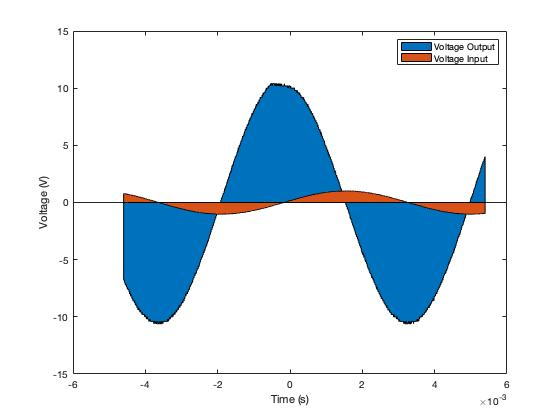
\includegraphics[width=10cm]{integral.jpg}\\\textbf{Graph 9}: From the collected raw data, this graph was constructed with the independent value $x$ being the time measured in seconds and the dependent value $y$ being the voltage. The blue area graph is the voltage output and the orange area graph is the voltage input. 
\end{center}
To confirm the theory of equation (22), the output voltage should equal to the $-\frac{1}{RC}$ of the integral of the input voltage. Thus, using the "trapz" function in MatLab the area under both graphs should equal to each other. The areas calculated were different but since the capacitor and the resistor are measured to be $10k\Omega$ and $10nF$, it helped making the right hand side of the equation equal the left hand side. The output voltage calculated by the equation (22) (Calculations found in Appendix) is $-0.012V$. 


\section*{Discussion and Conclusion}
To conclude, the experimental results satisfied the theoretical results. The purpose of this activity was to investigate various applications of op amps. The inverting and non inverting amplifiers gave an insight on the different and opposite oscillations when it comes to the output voltage. Theoretically when solving for the gain, equation (7) was used for the inverted amplifiers, while the equation (10) was used for the non inverted amplifiers. In both cases, the theoretical values from the resistors followed with the experimental values of the output amplitude and input amplitude. The experimental average error percentage between the amplitudes and the resistances gives a $0.83\%$ for the inverting amplifiers. Moreover, an average error percentage between the amplitudes and the resistances of non inverting amplifiers is $1.08\%$. Making the overall inverting and non inverting amplifiers a success, due to the following of the theory and the low error percentages.\\
According to multiple theories presented, equation (16) and equation(22) present themselves useful for the derivation of output voltage. Provided data and some computational analysis via matlab, the theory corresponded to the experimental performances. For the inverting differentiator, theoretically, it follows an output voltage of the negative resistance and capacitance of the derivative of the input voltage. Since the input followed a sine function, the derivative of that is cosine, giving a very accurate result via graph 7 in the discussion and analysis. For the inverting integrator, the theory follows the inverse of the resistor and capacitor time the integral of the input voltage. With the help of matlab and computational methods, the derived output of this circuit was $-0.012V$ in area under the curve. The experimental area under the curve of $-0.019V$ giving a $39\%$ error. Such high error could be due to the fact that the output was measured in millivolts affecting the calculations and forcing conversions. The input and output voltage graph had a difference of factor of 10, based on the calculations in the appendix, the results are close in theory but relatively could be redone to fit a better error percentage and calculations.\\
Overall, the experiment was a great success, investigating various applications of op amps helped research various information on op amps. The inverted and non inverted circuits were a great success. The inverted differentiation was successful due to the output voltage graph corresponding to the computational input voltage graph. Lastly, the inverted integrator could of been better for many reasons. Nonetheless, great laboratory experiment.

\newpage
\section*{Appendix}
Wagih, Ghobriel: Lab manual I: Introduction to Experimental Physics.\\
Figure 1: John M. Santiago Jr., PhD: Op Amp Circuits an Circuit Analysis.\\
"https://www.dummies.com/education/science/science-electronics/op-amp-circuits-and-circuit-analysis\\
PHY324 Advanced Physics Lab Manual, "Applications of Op Amps" \\
"http://hyperphysics.phy-astr.gsu.edu/hbase/Electronic/opampvar.html#c5"\\
ElectronicsTutorials\\
"https://www.electronics-tutorials.ws/opamp/opamp_2.html"\\

\begin{center}
\caption{Table 1: Table of Information for Inverting Amplifier} 
 \begin{tabular}{||c c c c c||} 
 \hline
 $\frac{V_o}{V_{in}}$ & $R_f$ & $R_{in}$ & $-\frac{R_f}{R_{in}}$ & Error Percentage \\ [0.5ex] 
 \hline\hline
 -9.394 & 98.1 & 10.57 & -9.28098 & 1.1962\%\\ 
 \hline
 -4.449 & 47.1 & 10.57 & -4.456 & 0.15709\%\\
 \hline
 -1.421 & 14.84 & 10.57 & -1.40397 & 1.2129888\%\\
 \hline
 -4.521 & 47.1 & 10.57 & -4.456 & 1.458707\%\\
 \hline
 -1.592 & 47.1 & 29.7 & -1.5858 & 0.3279102\%\\
 \hline
 -0.483 & 47.1 & 98.1 & -0.48 & 0.625\%\\ [1ex] 
 \hline
\end{tabular}
\\\textbf{Table 1}: This table contains the output voltage and input voltage recorded through matlab codes. Calculations of experimental gain and theoretical gain. Lastly, error percentages between theoretical and experimental gains. 
\end{center}
Calculation of theoretical gain of the first row:
\[-\frac{R_f}{R_{in}}=-\frac{98.1}{10.57}=-9.28098\]
Error percentage Calculation for the first row:
\[\frac{|theoretical-experimental|}{experimental}\cdot 100\% =\frac{|-9.394+9.28098|}{-9.394}\cdot 100\%=1.1962\%\]
Average error percentage:
\[\bar X= \frac{1}{n}\sum^n_{i\in\N}X_i=\frac{1.1962+0.15709+1.2129888+1.458707+0.3279102+0.625}{6}=0.829649 \%\]
\newpage
\begin{center}
    \textbf{Appendix Graph 1}: Oscilloscope Graph from Non Inverted Amplifier\\
    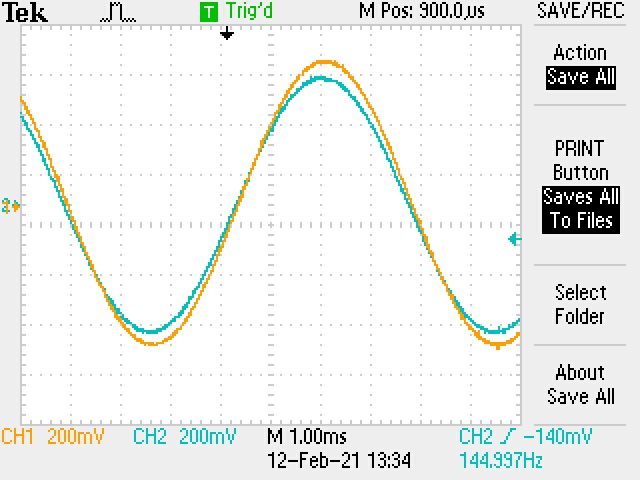
\includegraphics[width=10cm]{F0006TEK.JPG}\\\textbf{Appendix Graph 1}: This is an oscilloscope graph collected from the non inverted amplifier experiment. Compared to the inverted, it is not a negative of the input. Channel 1 is amplified after being initially inputted by channel 2. Channel 1 is the voltage output and channel 2 is the initial voltage. The independent axis is represented by the time in seconds. The dependent value is the voltage. 
\end{center}
\begin{center}
\caption{Table 2: Table of Information for Non-Inverting Amplifier} 
 \begin{tabular}{||c c c c c||} 
 \hline
 $\frac{V_o}{V_{in}}$ & $R_1$ & $R_2$ & $1+\frac{R_2}{R_1}$ & Error Percentage \\ [0.5ex] 
 \hline\hline
 1.11564 & 98.1 & 10.57 & 1.107747 & 0.7125273\%\\ 
 \hline
 1.231068 & 47.1 & 10.57 & 1.224416136 & 0.5432682\%\\
 \hline
 1.733215 & 14.84 & 10.57 & 1.712264151 & 1.2235758\%\\
 \hline
 1.242236 & 47.1 & 10.57 & 1.224416136 & 1.4553761\%\\
 \hline
 1.655715 & 47.1 & 29.7 & 1.630573248 & 1.5418965\%\\
 \hline
 3.114685 & 47.1 & 98.1 & 3.082802548 & 1.0342035\%\\ [1ex] 
 \hline
\end{tabular}
\\\textbf{Table 2}: This table contains the slopes collected from the output amplifier and input amplifier. The slope containing the experimental gain to compare it to the theoretical gain calculated with equation (10). As well as, error percentage between the theoretical and experimental gain.
\end{center}
Calculation of theoretical gain of the first row:
\[1+\frac{R_2}{R_1}=1+\frac{10.57}{98.1}=1.107747\]
Error percentage Calculation for the first row:
\[\frac{|theoretical-experimental|}{experimental}\cdot 100\% =\frac{|1.107747-1.11564|}{1.107747}\cdot 100\%=0.7125273\%\]
Average error percentage:
\[\bar X= \frac{1}{n}\sum^n_{i\in\N}X_i=\frac{0.7125273+0.5432682+1.22355758+1.4553761+1.5418965+1.0342035}{6}=1.085141233\%\]
\newpage
\begin{center}
    \textbf{Appendix Graph 2}: Oscilloscope Graph from Inverted Differentiator with Different Frequency\\
    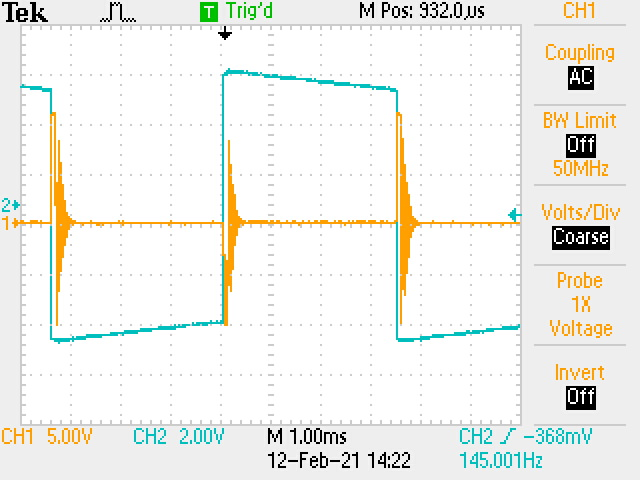
\includegraphics[width=7cm]{Differentiator/F0014TEK.JPG}
    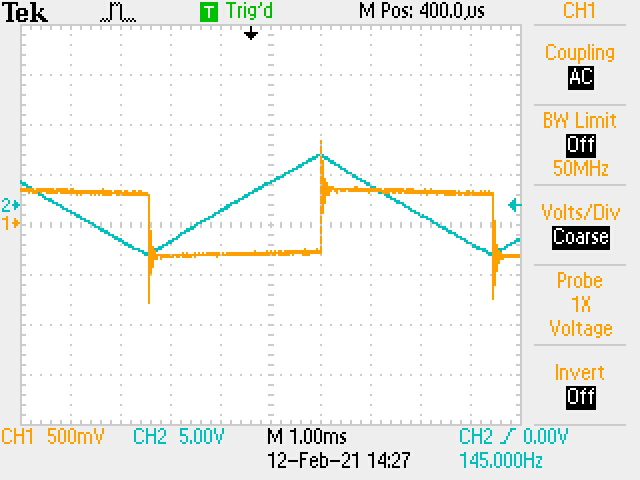
\includegraphics[width=7cm]{Differentiator/F0016TEK.JPG}
    \\\textbf{Appendix Graph 2}: This is an oscilloscope graph collected from the Inverted Differentiator. From the frequency change of 145Hz to 17Hz, there would be a lot of spikes in the graphs. 
\end{center}

Calculation of the derivation of Inverted Differentiator:
\[V_o=-RC\frac{dV_i}{dt}=-RC\frac{d(V_isin(\omega(t)))}{dt}=-RCcos(\omega t)\omega=-RCcos(\frac{1}{RC}t)(\frac{1}{RC})=-cos(\frac{1}{RC}t)\]


Area Calculation from Inverted Integrator:
\[v_o=\frac{1}{RC}\int^t_0v_i=\frac{1}{(10\cdot1000)(10\cdot10^{-9})}(-0.0012mV)=\frac{1}{(10\cdot1000)(10\cdot10^{-9})}(\frac{1}{1000})(-0.0012V)\]\[=\frac{10000}{1000}(-0.0012V)=10(-0.0012V)=-0.012V\]


\newpage
\begin{center}
    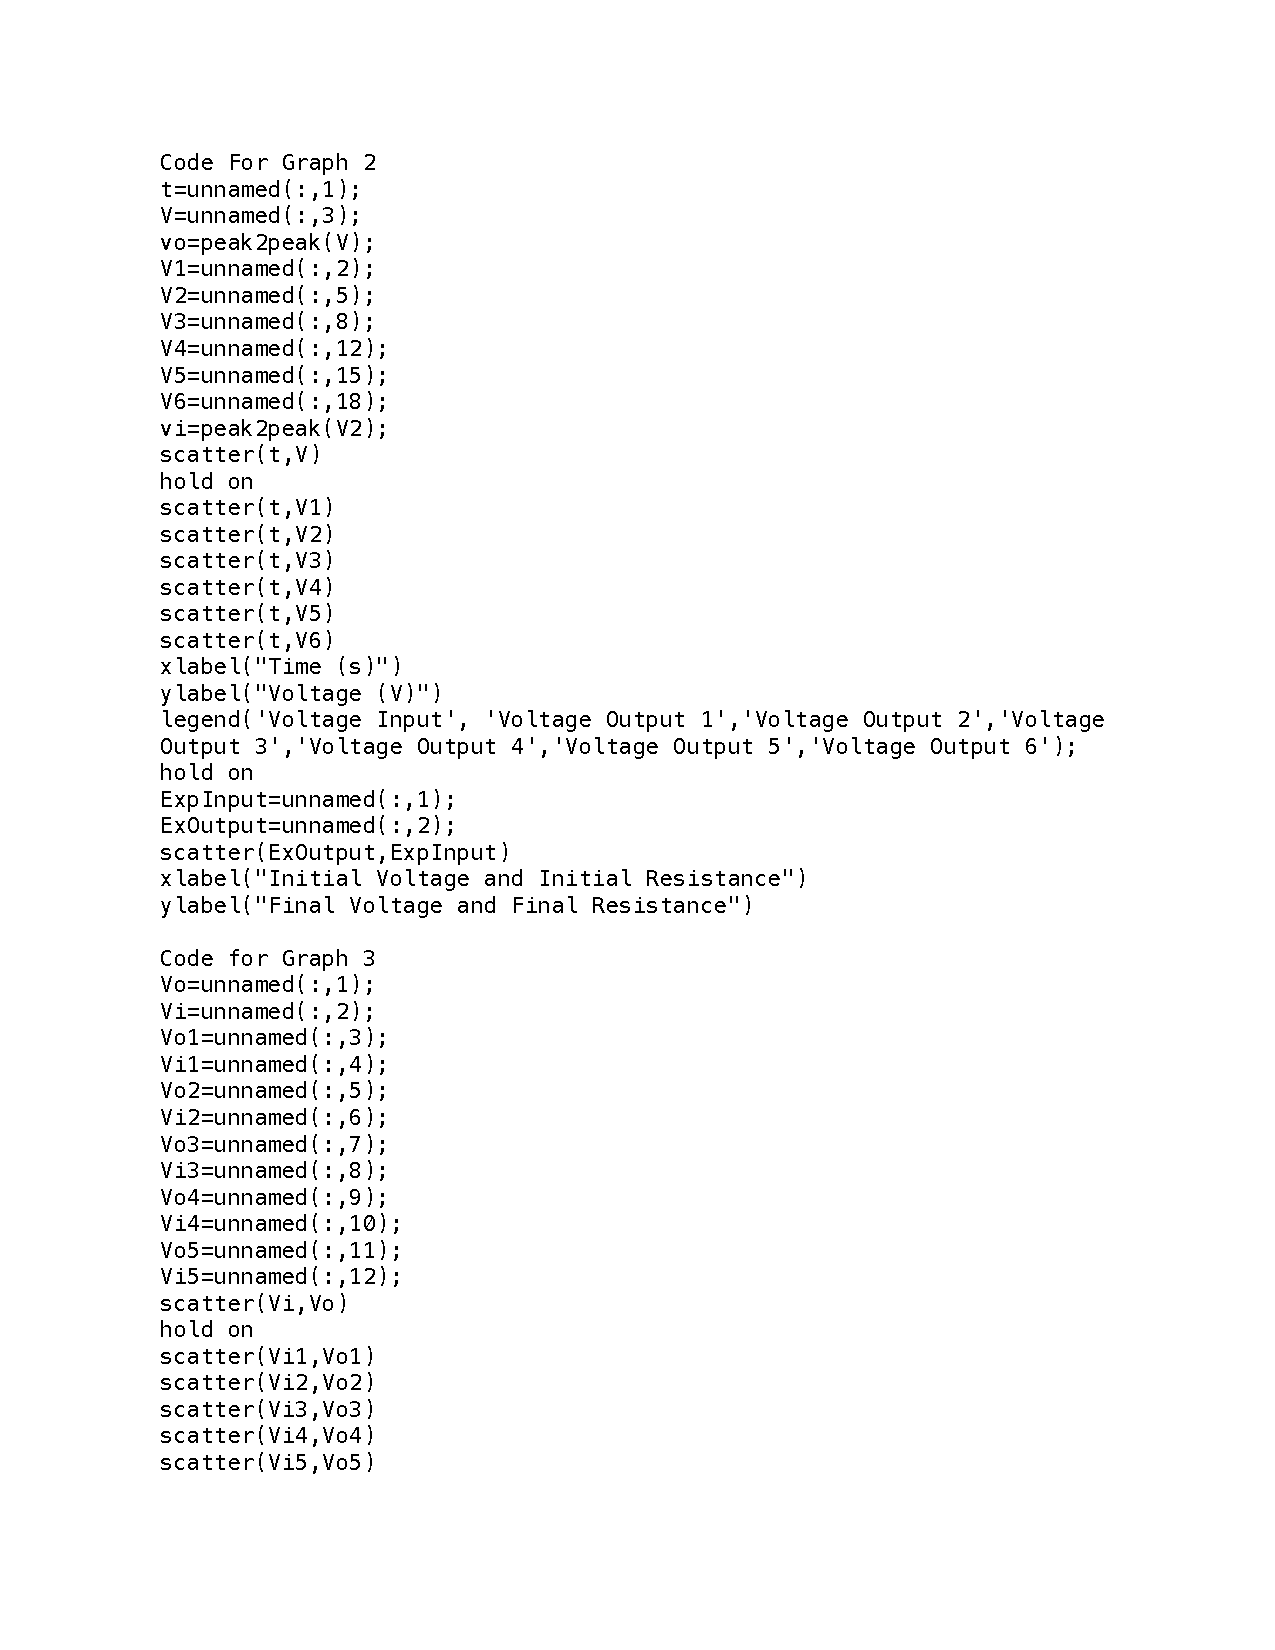
\includegraphics[width=15cm]{findingPeaks0.pdf}\\
    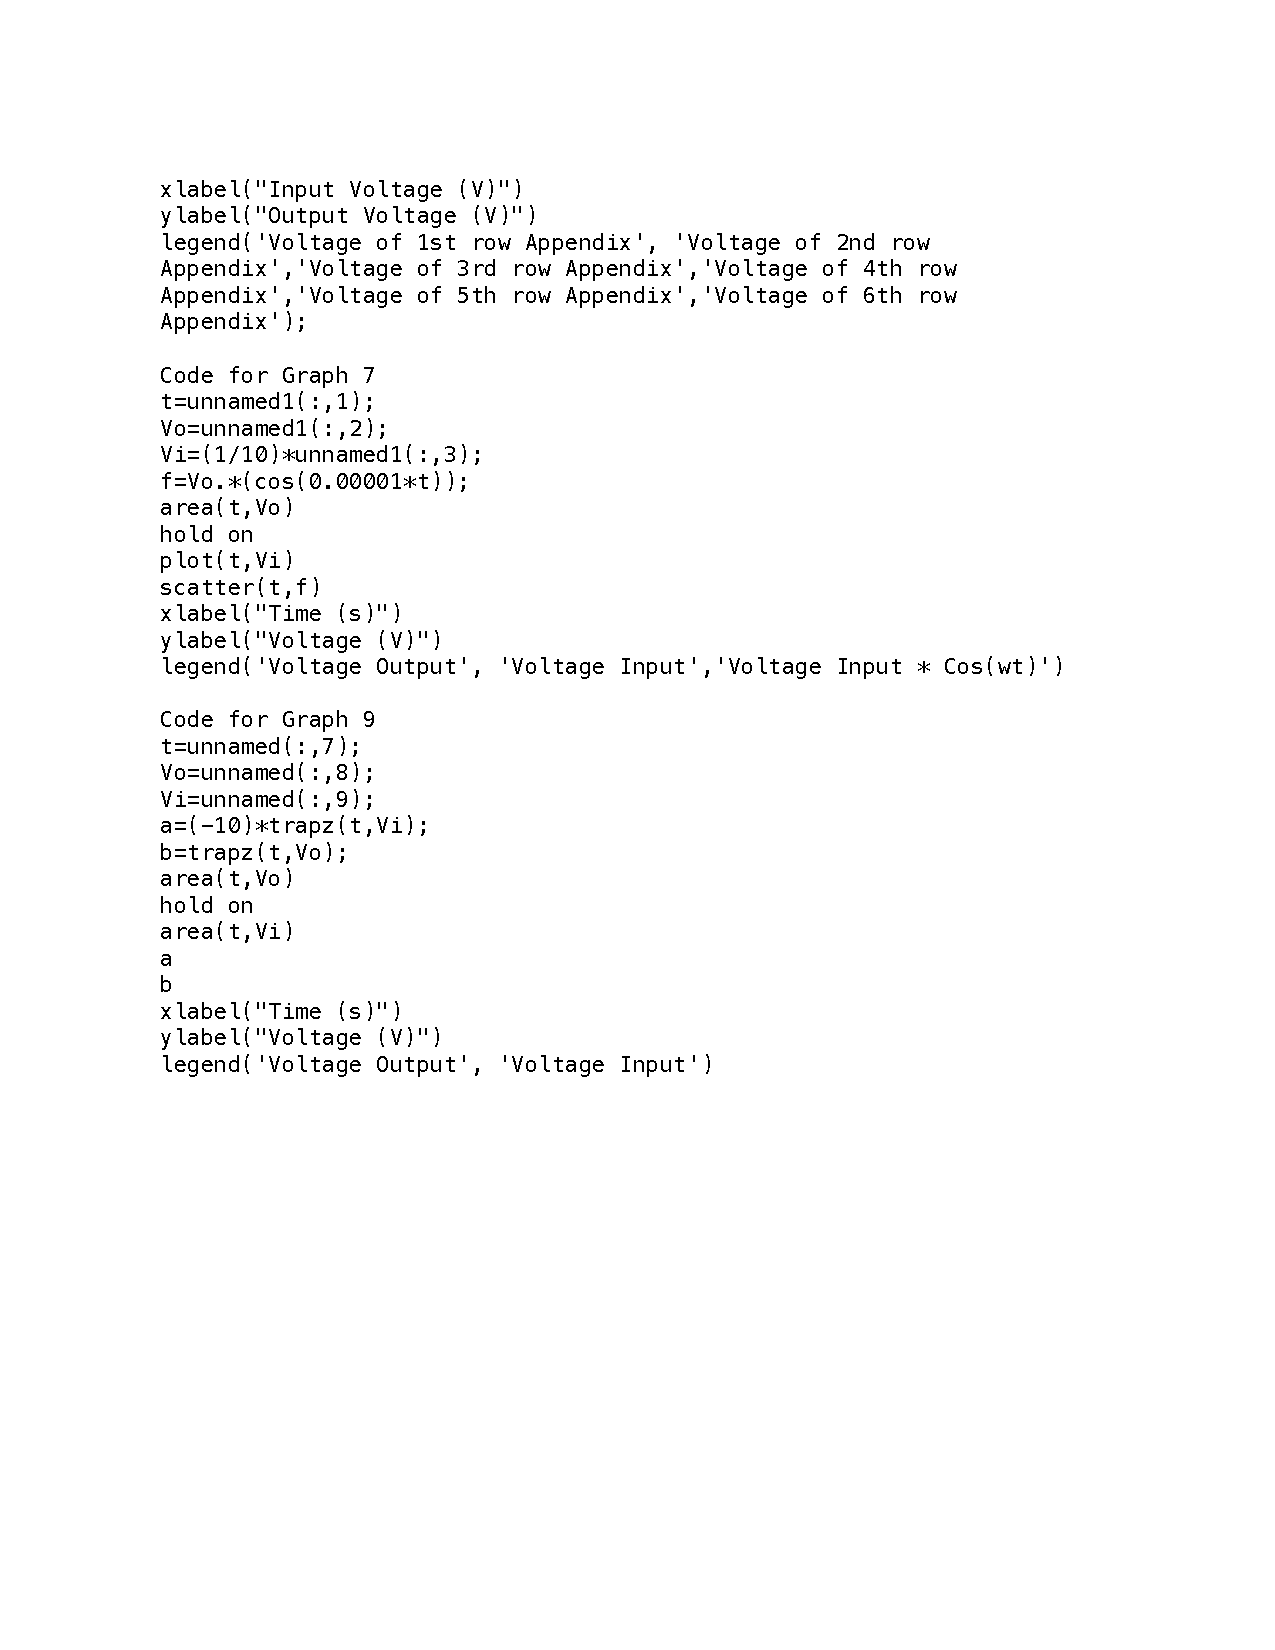
\includegraphics[width=15cm]{findingPeaks1.pdf}
    \\\textbf{Code}: These are the codes used in MatLab to generate the graphs.
\end{center}

\end{document}